\documentclass[12pt, a4paper]{article}
%%import package named hightest
\usepackage{hightest}
\usepackage{tikz}
%\usepackage{mathpazo}% change math font
%\usepackage[no-math]{fontspec}% font specfication
\header{រៀនគណិតវិទ្យាទាំងអស់គ្នា}{គណិតវិទ្យា}{\khmerdate}
\footer{រៀបរៀង និងបង្រៀនដោយ ស៊ុំ សំអុន}{ទំព័រ \thepage}{០៩៦ ៩៤០ ៥៨៤០}
\everymath{\protect\displaystyle\protect\color{black}}
\begin{document}
\maketitle
\begin{enumerate}[m]
	\item រូបភាព
	\begin{tikzpicture}
		\draw (0,0)	-- (4,0) -- (4,4) -- (0,4) -- (0,0);
	\end{tikzpicture}
	\item រូបភាព
	\begin{tikzpicture}
		\draw (0,0) -- (4,0) -- (4,4) -- (0,4) -- cycle;
	\end{tikzpicture}
	\item រូបភាព
	\begin{tikzpicture}
		\draw (0,0) rectangle (4,4);
	\end{tikzpicture}
	\item រូបភាព
	\begin{tikzpicture}
		\draw (0,0) parabola (4,4);
	\end{tikzpicture}
	\item រូបភាព 
	\begin{tikzpicture}
		\draw (0,0) .. controls (0,4) and (4,0) .. (4,4);
	\end{tikzpicture}
	\item រូបភាព
	\begin{tikzpicture}
		\draw (2,2) circle (2cm);
	\end{tikzpicture}
	\item រូបភាព
	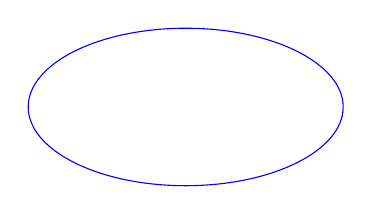
\begin{tikzpicture}
		\draw[blue] (2,2) ellipse (2cm and 1cm);
	\end{tikzpicture}
	\item រូបភាព
	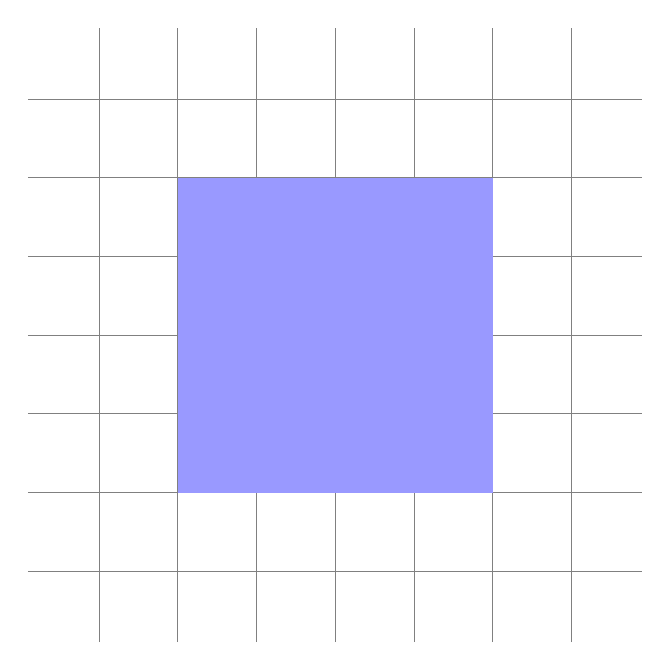
\begin{tikzpicture}
		\draw[step=1cm, gray, very thin] (-1.9,-1.9) grid (5.9,5.9);
		\fill[blue!40!white] (0,0) rectangle (4,4);
	\end{tikzpicture}
	\item រូបភាព
	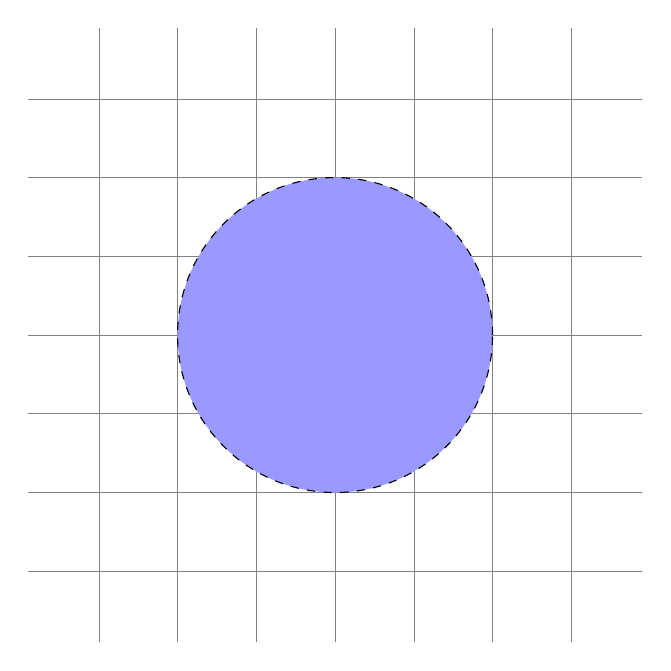
\begin{tikzpicture}
		\draw[step=1cm, gray, very thin] (-1.9,-1.9) grid (5.9,5.9);
		\fill[blue!40!white, dashed, draw=black] (2,2) circle (2cm);
	\end{tikzpicture}
	\item រូបភាព
	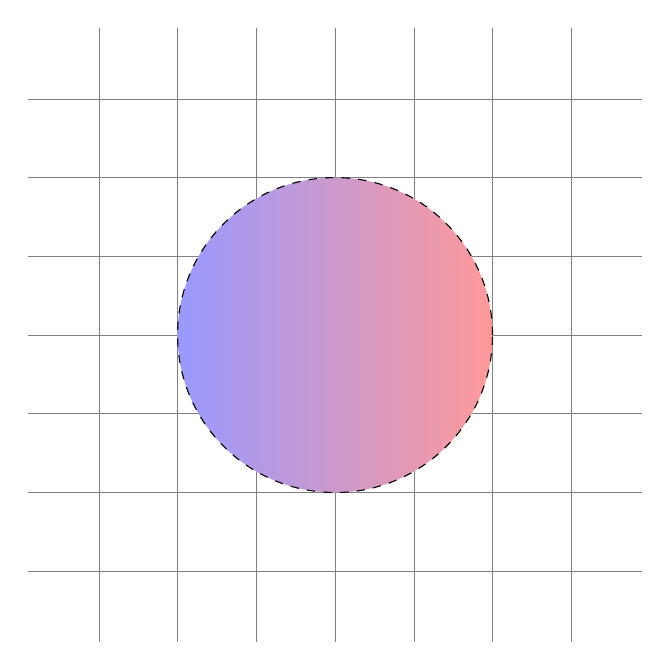
\begin{tikzpicture}
		\draw[step=1cm, gray, very thin] (-1.9,-1.9) grid (5.9,5.9);
		\shade[left color=blue!40!white, right color=red!40!white, dashed, draw=black] (2,2) circle (2cm);
	\end{tikzpicture}
	\item រូបភាព
	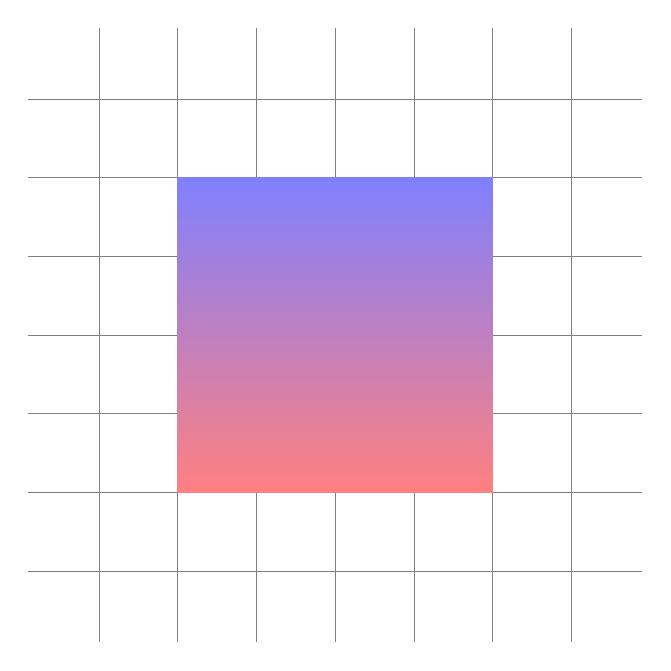
\begin{tikzpicture}
		\draw[step=1cm, gray, very thin] (-1.9,-1.9) grid (5.9,5.9);
		\shade[top color=blue!50!white, bottom color=red!50!white] (0,0) rectangle (4,4);
	\end{tikzpicture}
	\item រូបភាព
	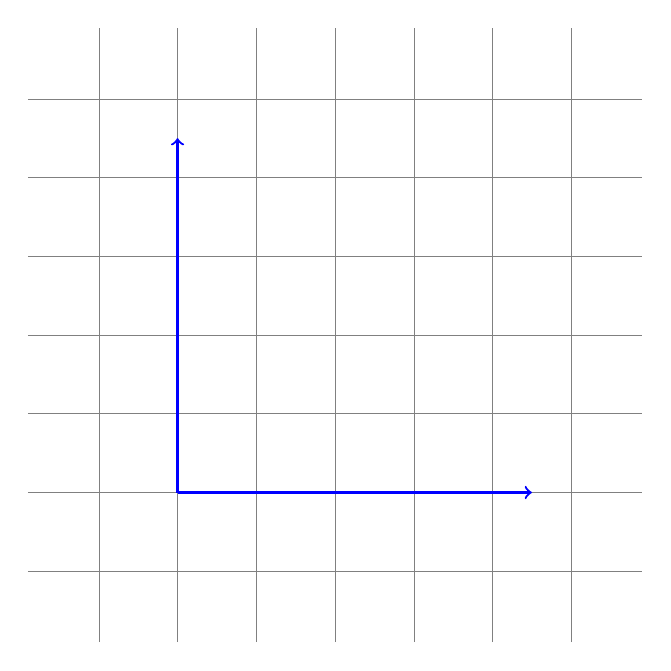
\begin{tikzpicture}
		\draw[step=1cm, gray, very thin] (-1.9,-1.9) grid (5.9,5.9);
		\draw[draw=blue,thick,->] (0,0) -- (4.5, 0);
		\draw[draw=blue,thick,->] (0,0) -- (0, 4.5);
	\end{tikzpicture}
	\item រូបភាព
	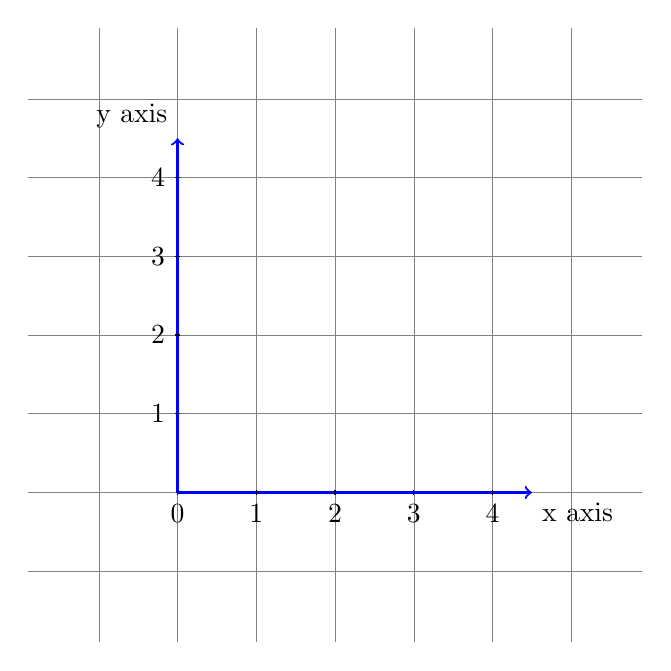
\begin{tikzpicture}
		\draw[step=1cm, gray, very thin] (-1.9,-1.9) grid (5.9,5.9);
		\draw[draw=blue,thick,->] (0,0) -- (4.5, 0)  node[anchor=north west] {x axis};
		\draw[draw=blue,thick,->] (0,0) -- (0, 4.5) node[anchor=south east] {y axis};
		\foreach \x in {0,1,2,3,4}
		\draw (\x cm,1pt) -- (\x cm,-1pt) node[anchor=north] {$\x$};
		\foreach \y in {1,2,3,4}
		\draw (1pt,\y cm) -- (-1pt,\y cm) node[anchor=east] {$\y$};
	\end{tikzpicture}
\end{enumerate}
	\begin{center}
		\sffamily\color{black}
		សូមសំណាងល្អ!
	\end{center}\newpage
\end{document}